\documentclass[aps, prc, reprint, amsmath, groupedaddress, nofootinbib]{revtex4-1}
\usepackage[compat=1.1.0]{tikz-feynman}
\usepackage[utf8]{inputenc}
\usepackage{hyperref}
\usepackage{amsmath}
\usepackage{amssymb}
\usepackage{amsfonts}
\usepackage{tabularx}
\usepackage{booktabs}
\usepackage{graphicx}
\usepackage{color}
\usepackage{multirow}
\usepackage[inline]{enumitem}
\graphicspath{{fig/}}
\definecolor{theblue}{RGB}{0,50,230}
\usepackage{appendix}
\hypersetup{
  colorlinks=true,
  linkcolor=theblue,
  citecolor=theblue,
  urlcolor=theblue
} 



\newcommand{\trento}{T\raisebox{-0.5ex}{R}ENTo}
\newcommand{\nch}{N_\text{ch}}
\newcommand{\sqrts}{\sqrt{s_{NN}}}
\newcommand{\T}{\tilde{T}}
\newcommand{\paddedhline}{\noalign{\smallskip}\hline\noalign{\smallskip}}
\newcommand{\dnchdy}{dN_\text{ch}/d\eta}
\newcommand{\dndypP}{dN_\text{pPb}/d\eta}
\newcommand{\dndyPP}{dN_\text{PbPb}/d\eta}
\newcommand{\x}{\mathbf x}
\newcommand{\y}{\mathbf y}
\newcommand{\z}{\mathbf z}
\newcommand{\trans}{^\intercal}

\newcommand{\Raa}{R_{AA}}
\newcommand{\vv}{v_2\{2\}}
\newcommand{\vvv}{v_3\{2\}}
\newcommand{\vnv}{v_n\{2\}}
\newcommand{\ppi}{\frac{\partial}{\partial p_i}}
\newcommand{\ppj}{\frac{\partial}{\partial p_j}}
\newcommand{\ppl}{\frac{\partial}{\partial p_l}}
\newcommand{\Kpara}{\kappa_{\|}}
\newcommand{\Kperp}{\kappa_{\perp}}
\newcommand{\Ppara}{\hat{P}^{\|}}
\newcommand{\Pperp}{\hat{P}^{\perp}}

\begin{abstract}
Current observation of open charm in heavy-ion collisions shows unexpectedly large momentum anisotropy and small nuclear modification factor, posing a challenge to the theoretical understanding of the nature of coupling between heavy quark and the medium.
Linear Boltzmann transport and Langevin diffusion are two popular kinetic models for heavy quark in-medium propagation.
In this work, we develop a hybrid heavy quark transport model that combines the strengths of both: 
heavy quarks are evolved with Langevin diffusion using an empirical diffusion constant and scattering processes treated linear Boltzmann equations with perturbative matrix elements.
The Langevin component is a complementary contribution to the linear Boltzmann equation when perturbative scattering is inadequate.
Both elastic and inelastic scatterings are included in the Boltzmann component.
The Landau-Pomeranchuk-Migdal effect is treated effectively via gluon formation time and detailed balance is imposed between gluon emission and absorption.
With the hybrid model, we study the heavy flavor momentum anisotropic, nuclear modification factor, and correlation observables in A-A collisions at the RHIC and the LHC energies.
Comparing to available D and B meson data, we constrain the diffusion constant of the Langevin component.

\end{abstract}


\begin{document}


\title{A hybrid heavy quark transport model in a quark-gluon plasma that couples linear Boltzmann equation and Langevin diffusion dynamics}
\author{Weiyao Ke}
\author{Yingru Xu}
\author{Steffen A.\ Bass}
\affiliation{Department of Physics, Duke University, Durham, NC 27708-0305}
\date{\today}
\maketitle

\section{Introduction}
In recent years, Relativistic Heavy-Ion Collider (RHIC) at Brookhaven National Laboratory and later the Large Hadron Collider (LHC) at CERN discovered a new state of matter, namely the strongly coupled quark-gluon plasma (sQGP), in ultra-relativistic heavy-ion collisions.
Two key signatures in the discoveries of sQGP are the collective flows and the jet quenching.
The collective flows reveal the surprising fact that the bulk medium of sQGP undergoes a strong collective expansion after being produced and the behaviors can be explained in great details by viscous hydrodynamics with the smallest specific viscosity ($\eta/s$) ever discovered in nature.
The jet quenching refers to that the yield of high transverse momentum hadrons in nuclear collisions are strongly suppressed compared to the yield in proton proton collision where medium effects should be small.
Calculations have shown that this suppression is a consequences of jet losing energy to the hot, dense and color-deconfined medium. 

Open heavy flavors (charm and bottom) as probes of sQGP partly belong to the jet observables but they are also unique because of the large masses and flavors.
Since the temperatures achieved in the experiments are still much smaller than charm and bottom masses, their thermal productions are highly suppressed; 
therefore the dominant production mechanism is production through initial hard process.
Heavy flavors are rare in heavy ion collisions even at low transverse momentum due to the mass, so they barely annihilate or recombine with their anti-particles, roughly conserving its number during the time-scale of sQGP.
These two features are particular attractive to theorists as heavy quarks experienced the medium full-time evolution and flavor-tagged particles are much easier to track in the calculations than the evolution of a full jet.
Finally, the mass sets an additional energy scale to the problem and brings rich physics to the heavy flavor sector.
In the high transverse momentum region, heavy quarks lose energy mainly through radiative process and this merge into the regime of jet energy loss study;
in the low momentum region, mass effect delays its thermalization time, providing a window to study the equilibration process.
Heavy flavors are therefore an ideal and unique probe to study the sQGP properties.

The in-medium propagation of heavy flavors is often studied in a kinetic approach that is linearized with respect to heavy quark distribution function. 
This linearization means any back reactions from heavy quark to the medium are neglected.
Linearized Boltzmann transport equation and Langevin equation are both widely used linearized models but focus on different levels of description of the interaction.
The linearized Boltzmsport equation is built on elementary scattering processes that can be directly related to fundamental calculations.
In principal, perturbative-QCD (pQCD) can predict the cross-section of these elementary scatterings.
However, these calculation in the presence of a medium is extremely complicated even at leading order.
Also, the pQCD processes are often plagued by soft divergence that need to be regulated by a medium scale proportional to the temperature, but with current collision energies the relevent temperature scale is not high enough that brings large ambiguity to pQCD calculation through the scale dependence of the strong coupling constant $\alpha_s(\mu T)$.
The Langevin equation takes a different perspective. 
It assumes that heavy quark receives frequent but soft momentum kicks from the medium, then a statistical description in terms of "drag" and "diffusion" coefficients of the interaction is possible.
These transport coefficients encode the first and second momentums of the momentum exchange rate but are agnostic to further details of the elementary processes.
One can again evaluate these transport coefficients from first principals, but for us focusing on learning these properties from experiment data, it is the vast flexibility to parametrize these quantities that the Langevin equation is most useful.
Of course, in this way it is not clear how to establish a direct relation between the extracted values and a more fundamental understanding.
In this work, we would like to combine the strengths of both approaches
and we have developed a hybrid heavy quark transport model described as follows.
The heavy quark scatters off medium particles in a linear Boltzmann equations with pQCD matrix elements (the scattering component), and between scatterings heavy quark is propagated by a Langevin equation (the diffusion component) with empirical transport coefficient mimicing the interaction missing from the above scattering picture.
Both elastic and inelastic scatterings are included in the scattering component with soft divergence screened by a Debye mass $m_D^2 \sim \alpha_s T^2$ and Landau-Pomeranchuk-Migdal (LPM) effect taken into account effectively.
The renormalization scale $\mu$ is the only parameter in the scattering component and the diffusion component has several parameters which carries an implicit dependence on $\mu$ once we tuned the model to data.
The effect of small momentum transfer scatterings that may suffer too much from the scale ambiguity is assumed to be compensated by the diffusion component. 
In addition, the diffusion component may conceptually receive other diffusion-like contributions such as non-perturbative effects.
We have noticed that a rigorous separation of matrix-element scattering and diffusion has been proposed for the study of jet energy loss up to next-to-leading order within the context of pQCD.
In our study, we don't require the content of the diffusion component to be pQCD in nature.
In fact, we can understand this hybrid approach in the following way, given that a major part of the heavy quark medium interaction is explained by pQCD, what is still needed for the theory to describe the data is parameterized in diffusion component that can be learned from data.

To learn the knowledge in the context of relativistic heavy-ion collisions, we calibrated all model parameters by comparing model calculation to experimental data to see how the system must behave.
The calibration involves evaluating a multi-stage and multi-component model of the medium plus heavy flavor evolution over a high dimensional parameter space.
The dimensionality of the problem makes it impossible to be tuned by hands.
To solve this problem, our group have been developing powerful statistical tools based on Bayesian methodology to conduct systematic model to data comparisons.
This approach treats experimental uncertainties seriously and explores the probability likelihood function of the model parameters given the experimental data.
Usually among all the parameters, some parameters are physical such as transport coefficients and others are non-physical such as cut-off parameters. 
And very often, we are interested in a few or a certain combination of the physical parameters.
For this purpose, the Bayesian technique marginalizes over (integrates out) other parameters and computes the probability distribution for the parameters of interest. 
The marginalization provides a parameter range that is not only preferred by the experiments, but also already includes uncertainties of in the marginalized parameters.
Therefore the Bayesian technique really tells what can be actually learned from the data, considering both experimental accuracy and model parameter uncertainties.
This procedure has been successfully applied to extracting initial condition and bulk transport coefficients from soft observables and to the heavy quark sector extracting heavy quark momentum diffusion parameter $\hat{q}$ using a radiation improved Langevin equation.
In this work, we provide another extraction of heavy quark transport properties using the hybrid model and demonstrate how the use of different models affects the results of parameter extraction.

The paper is organized as follows. We describe the hybrid model in detail in section \ref{section:model}. In section \ref{section:test}, the model is tested in a static medium to provide straightforward characterization. We calibrate the model parameters in section \ref{section:calibration} and with high likelihood parameter sets novel observables are predicted in section \ref{section:prediction}. Finally, section \ref{section:conclusion} contains summary and discussion of results.

\section{Heavy quark propagation in a hybrid transport model}\label{section:model}
\subsection{Scattering component}
Elementary scatterings of heavy-flavor with medium particles are treated in a linearized Boltzmann equation,
\begin{eqnarray}
  \frac{\partial}{\partial t}f_Q - \frac{\vec{p}}{E}\cdot\nabla f_Q  = 
\mathcal{C}[f_Q]
%C_i^{2\rightleftharpoons 2}[f_Q] + C_i^{2\rightleftharpoons 3}[f_Q]
\end{eqnarray}
The left hand side represents free transport of the heavy quark distribution function. 
Scatterings with medium partons change the distribution via the collision integral on the right.
The medium parton distribution function are assumed to follow a Maxwell--J\"uttner distribution, 
\begin{eqnarray}
f_{q,\bar{q}, g} = \exp\left(-\frac{p \cdot u(x)}{T(x)}\right),
\end{eqnarray}
and any off-equilibrium corrections to the medium partions are neglected.
The space-time evolution of the temperature field $T$ and velocity field $u^\mu$ are obtained in an event-by-event 2+1D viscous relativistic hydrodynamic calculation.
We solve $f_Q(x, p, t)$ in a Monte Carlo way by representing the distribution function with an ensemble of heavy quarks.
Each heavy quark can freestream or scatter within a given time step $dt$.
In each collision, the heavy quark collide a few medium particles that together forms an $n$-body initial state $\{\textrm{in}\}$, and the outgoing particles after the collision forms the $m$-body final satte $\{\textrm{out}\}$.
The scattering probability $P$ of a certain channel for a heavy quark with energy $E_1$ inside a medium with temperature $T$ from $t$ to $t+dt$ is calculated from the scattering rate $R$,
\begin{eqnarray}\label{eq:rate}
    P(E_1,T,t,dt) &=& R(E_1, T, t) dt \\
    &=& \frac{d}{\nu} \frac{\delta}{\delta f_Q(p_1)}\int d \Gamma \prod_{\textrm{\{in\}}} f_i(p_i) 
\overline{|M|^2},
  	 \nonumber
\end{eqnarray}
where the $d\Gamma$ is the $(n+m)$-body phase-space integration,
\begin{eqnarray}
\nonumber
d\Gamma = (2\pi)^4\delta^4\left(\sum_{\textrm{\{in\}}}p_{i} - \sum_{\textrm{\{out\}}}p_{i}\right)\prod_{\{\textrm{in, out}\}} \frac{dp_i^3}{2E_i(2\pi)^3} 
\end{eqnarray}
$\overline{|M|^2}$ is the initial state spin-color averaged scattering matrix-element square.
$d$ counts the degeneracy of the incoming medium particle and $\nu$ is the symmetry factor of identical gluons in the initial / final state of the collision.
If one determines heavy quarks scatters via certain channel within $dt$ according to the probablity $P$, the details of the initial and final states can be obtained by sampling the differential scattering rate over the phase space.
The time step $dt$ is chosen small enough so that the probability of multiple scatterings within $dt$ is negligible. 

Now, we focus on what processes to be included in the collision term.
It has been shown that at lowest order in the coupling constant, heavy quarks can scatter elastically with light parton (quark, anti-quark or gluon) or emitting collinear gluon triggered by soft collisions which we call an inelastic process based on its particle number changing nature.
We will keep use the term ``elastic" and later ``inelastic" to distinguish these two types of processes and their associated energy loss.
For quark-gluon scattering, there are three diagrams corresponds to $s, t,$ and $u$ channel exchange; only $t$ channel contributes to quark-quark scattering as shown in Fig. \ref{plots:feyn-elastic}.
The matrix-elements for these processes in vacuum are available at leading order pQCD (see \ref{appendix:matrix-element}).
In these expressions, the characteristic $t-$channel gluon propagator causes divergence in cross-section as the momentum transfer vanishes,
\begin{eqnarray}
d\sigma \propto \frac{1}{t^2} dt.
\end{eqnarray}
But inside a quark-gluon plasma, those soft exchanging gluon will constantly interact with medium particles and this divergence should be  screened by a Debye mass in the case of static scattering center.
Generally, the gluon propagator should be replaced by a hard-thermal loop (HTL) propagator.
But this HTL propagator involves a complicated self energy that depends on the medium reference frame, so it is hard for us to apply it in a cross-section based Monte-Carlo approach where it is easiest to calculate and sample in the two- or three-body center of mass frame.
Hence we choose to adopt the simple replacement $t^2 \rightarrow (t-\Lambda_{QCD}^2)(t - m_D^2)$ (up to an additional $\Lambda_{QCD}^2$) that taken into account dynamical medium effects.
At high energy, inelastic processes shown in Fig. \ref{plots:feyn-inelastic} becomes important.
Although it seems to be one order higher in coupling constant than the elastic processes, because of the divergence in emitting soft gluon which we screened by the asymptotic gluon thermal mass $m_D/\sqrt{2}$, it actually contributes at the same order as elastic energy loss.
The available phase space for radiating a gluon also grows with heavy quark incident energy and it eventually becomes the dominate energy loss mechanism at high energies.
Boltzmann equation with only the gluon radiation ($2\rightarrow 3$) process violates detailed balance, we also include the reverse process namely the medium gluon absorption ($3\rightarrow 2$) process so that the model approaches the correct thermal equilibrium at large time.
The matrix-element for the absorption relates to the radiation matrix-element by sending the final state gluon emission line to the initial state ($k^\mu \rightarrow -k^\mu$).
This medium gluon in the initial state brings an additional Boltzmann factor $e^{-k/T}$ and it is not easy for a fast moving heavy quark to absorb a low energy gluon, so we expect it to be less relevant for high incident energy heavy quarks propagates in low temperature medium. 
But this is essential for the region close to thermalization when low energy heavy quark effectively absorbs gluon with $k \sim T$.
We shall study numerically in the next section to answer under what conditions the medium gluon absorption process is important.

A complication for inelastic processes is that the radiated (absorbed) gluon takes finite amount of time to be fully resolved from (merged into) the heavy quark.
This typical time scale is called the gluon formation time $\tau_f$, during which the effects of multiple soft collisions add up coherently in a destructive way to suppress the gluon emission spectrum.
This is known know as the LPM effect.
The formation time for a heavy quark to radiate a gluon is,
\begin{eqnarray}
\tau_f &=& \frac{2x(1-x)E}{k_\perp^2 + x^2M^2 + (1-x)m_D^2/2}, x = \frac{k^+}{E^+}
\end{eqnarray}
The gluon emission probability now dependents on multiple collisions along the trajectory of the heavy quark and the problem becomes non-local.
This is particularly difficult to implement in the collision term of the linearized Boltzmann equation, because all scatterings are treated as localized in space-time.
In our model, we mimic the LPM effect by restricting the phase space integral of this additional gluon with a coherence factor,
\begin{eqnarray}
d\Gamma_k \rightarrow 2\left(1 - \cos\left(\Delta t/\tau_f\right) \right)d\Gamma_k,
\end{eqnarray}
where $\Delta t$ is the time elapsed from the last radiation.
This factor is determined by requiring that the differential radiation rate reduces to the formula used by [] when gluon transverse momentum is much large than the momentum transfer from medium ($k_\perp^2 \gg q_\perp^2$).
With this prescription, gluon with formation time is greater than $\Delta t$ is suppressed, at the expense that the collision rate becomes history dependent.
It is not trivial to tell if the Boltzmann equation with a history-dependent rate should thermalize as $t\rightarrow \infty$, so we test and confirm the model approaches correct thermal limit in the next section.

\begin{figure}
\feynmandiagram [xscale=.95, yscale=1, horizontal=a to b] {
  p1 -- [fermion] a--b[fermion] -- [fermion] p3 ,
  p2 -- [gluon] a,
  p4 -- [gluon] b,
};
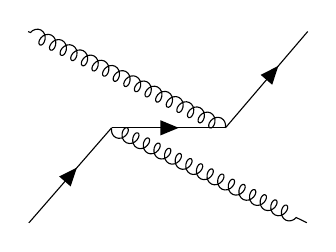
\begin{tikzpicture}[xscale=.95, yscale=1.]
  \begin{feynman}
    \diagram [horizontal=a to b] {
      i1 %[particle=\(Q\)]
      -- [fermion] a
      -- [draw=none] f1,% [particle=\(g\)],
      a -- [fermion] b,
      i2 %[particle=\(Q\)]
      -- [anti fermion] b
      -- [draw=none] f2,% [particle=\(g\)],
    };
    \diagram* {
      (a) -- [gluon] (f2),
      (b) -- [gluon] (f1),
    };
  \end{feynman}
\end{tikzpicture}
\feynmandiagram [xscale=1.2, yscale=.8, horizontal=p2 to p4] {
  p2 [particle=$g$]-- [gluon] b -- [gluon] p4 [particle=$g$],
  a -- [gluon] b,
  p1 [particle=$Q$] -- [fermion] a -- [fermion] p3 [particle=$Q$],
};
\feynmandiagram [xscale=1.2, yscale=.8, horizontal=p1 to p3] {
  p2 [particle=$q$] -- [fermion, edge label=$p_2$] a -- [fermion, edge label=$p_4$] p4 [particle=$q$],
  a -- [gluon, momentum=$q$] b,
  p1 [particle=$Q$] -- [fermion, edge label=$p_1$] b -- [fermion, edge label=$p_3$] p3 [particle=$Q$],
};
\caption{Elastic processes. The first three diagrams contribute to heavy quark (Q) - gluon (g) scattering, the last one contributes to a light (anti-)quark (q) scattering. Intermediate propagators are screened by a Debye mass in case of soft divergence.}\label{plots:feyn-elastic}
\end{figure}

\begin{figure}
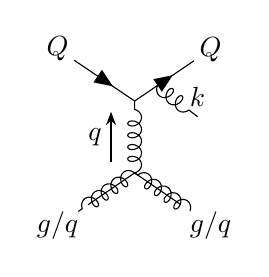
\begin{tikzpicture}
  \begin{feynman}
    \diagram [xscale=0.8, yscale=.6, vertical=a to b] {     
      i2 [particle=\(g/q\)]
        -- [gluon] b
        -- [gluon] f2 [particle=\(g/q\)]],
      b -- [gluon, momentum=$q$] a,
      i1 [particle=\(Q\)]
        -- [fermion] a
        -- [fermion] f1 [particle=\(Q\)],
    };
    \vertex [below right=.2 cm and .8 cm of a, label=\(k\)] (r);
    \draw [gluon] ($(a)!0.3!(f1)$) -- (r);
    \draw  (i2)--(b);
     \draw  (b)--(f2);
  \end{feynman}
\end{tikzpicture}
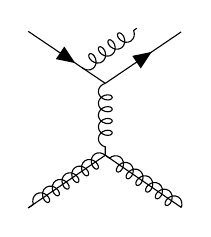
\begin{tikzpicture}
  \begin{feynman}
    \diagram [xscale=0.8, yscale=0.6, vertical=a to b] {     
      i2  -- [gluon] b
        -- [gluon] f2,
      a -- [gluon] b,
      i1 -- [fermion] a
        -- [fermion] f1,
    };
    \vertex [above right=.7 cm and .4 cm of a] (r);
    \draw [gluon] ($(i1)!0.7!(a)$) -- (r);
    \draw  (i2)--(b);
     \draw  (b)--(f2);
  \end{feynman}
\end{tikzpicture}
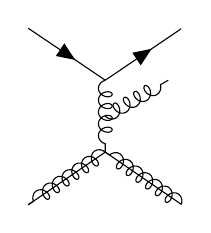
\begin{tikzpicture}
  \begin{feynman}
    \diagram [xscale=0.8, yscale=.6, vertical=a to b] {     
      i2 %[particle=\(g\)]
        -- [gluon] b
        -- [gluon] f2, %[particle=\(g\)]],
      a -- [gluon] b,
      i1 %[particle=\(Q\)]
        -- [fermion] a
        -- [fermion] f1, %[particle=\(Q\)],
    };
    \vertex [below right=.0 cm and .8 cm of a] (r);
    \draw [gluon] ($(a)!0.5!(b)$) -- (r);
    \draw  (i2)--(b);
     \draw  (b)--(f2);
  \end{feynman}
\end{tikzpicture}
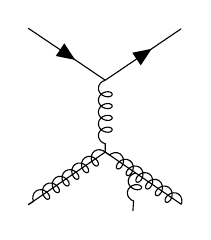
\begin{tikzpicture}
  \begin{feynman}
    \diagram [xscale=0.8, yscale=.6, vertical=a to b] {     
      i2 %[particle=\(g\)]
        -- [gluon] b
        -- [gluon] f2, %[particle=\(g\)]],
      a -- [gluon] b,
      i1 %[particle=\(Q\)]
        -- [fermion] a
        -- [fermion] f1, %[particle=\(Q\)],
    };
    \vertex [below right=.75 cm and .35 cm of b] (r);
    \draw [gluon] ($(i2)!0.6!(b)$) -- (r);
    \draw  (i2)--(b);
     \draw  (b)--(f2);
  \end{feynman}
\end{tikzpicture}
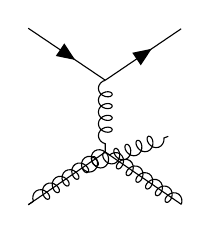
\begin{tikzpicture}
  \begin{feynman}
    \diagram [xscale=0.8, yscale=.6, vertical=a to b] {     
      i2 %[particle=\(g\)]
        -- [gluon] b
        -- [gluon] f2, %[particle=\(g\)]],
      a -- [gluon] b,
      i1 %[particle=\(Q\)]
        -- [fermion] a
        -- [fermion] f1, %[particle=\(Q\)],
    };
    \vertex [above right=.2 cm and .8 cm of b] (r);
    \draw [gluon] ($(b)!0.3!(f2)$) -- (r);
    \draw  (i2)--(b);
     \draw  (b)--(f2);
  \end{feynman}
\end{tikzpicture}
\caption{Inelastic process. Heavy quark collide with a meidum light (anti-)quark or gluon and radiates an additional gluon.}\label{plots:feyn-inelastic}
\end{figure}

\subsection{Diffusion component}
The diffusive motion of heavy quarks are solved in Langevin equations in terms of drag and diffusion.
The Langevin equations in the Ito scheme are,
\begin{eqnarray}
\Delta \vec{x}_i &=& \frac{\vec{p}_i}{E} \Delta t	\\
\Delta \vec{p}_i &=& -\Gamma \vec{p}_i \Delta t + \Delta t \vec{\xi}
\end{eqnarray}
The first equation is the transport part.
The second equation changes the momentum by a drag term with coefficient $\Gamma$ and a thermal random force $\vec{\xi}$. 
The random force has zero mean and the covariance structure:
\begin{eqnarray}
\langle \xi_i \xi_j \rangle = \frac{1}{\Delta t}\left(\Kpara \frac{p_i p_j}{p^2} + \Kperp \left(\delta_{ij} - \frac{p_i p_j}{p^2}\right) \right)
\end{eqnarray}
In this study, we assume the diffusion component is isotropic $\Kpara=\Kperp=\kappa$.
The drag coefficient $\Gamma$ and the momentum diffusion coefficient $\kappa$ need to satisfy the Einstein relation in Ito scheme to guarantee reaching the correct thermal equilibrium at large time,
\begin{eqnarray}
\Gamma &=& \frac{\kappa}{2TE} - \frac{d\kappa}{dp^2}
\end{eqnarray}
We choose momentum diffusion $\kappa$ as the independent variable in our parametrization.
If temperature is the only scale in the problem, we expect $\kappa$ to scale as $T^3$.
Additional, we consider the possibility of non-perturbative contribution to the diffusion component, which only happens at low energy and low temperature and we arrive at this simple ansatz,
\begin{eqnarray}
\frac{\kappa}{T^3} = A\left(x + (1-x)\frac{[1\textrm{ GeV}]^2}{ET}\right)
\end{eqnarray}

\section{Tests in a static medium}\label{section:test}
\begin{figure}
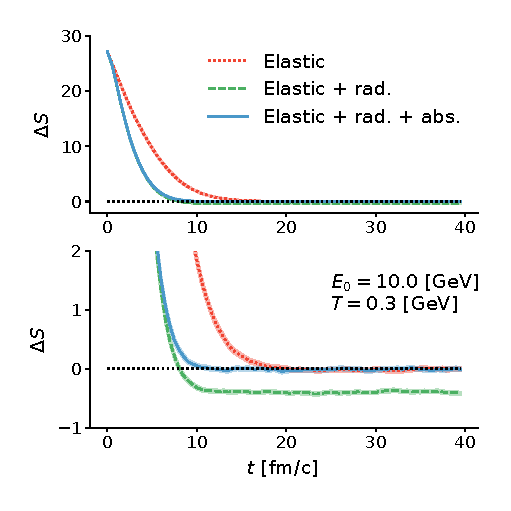
\includegraphics[width=\columnwidth]{thermalization.pdf}
\caption{The approach to thermalization of the linear Boltzmann equation with elastic processes only (red dot), elastic with radiation processes (green dashed), and elastic with both radaition and absorption processes (blue solid). The static medium has a temperature $T = 0.4$ GeV. $10^4$ heavy quarks are initialized with $E = 10$ GeV at $t = 0$.}\label{plots:thermalization}
\end{figure}
\begin{figure*}
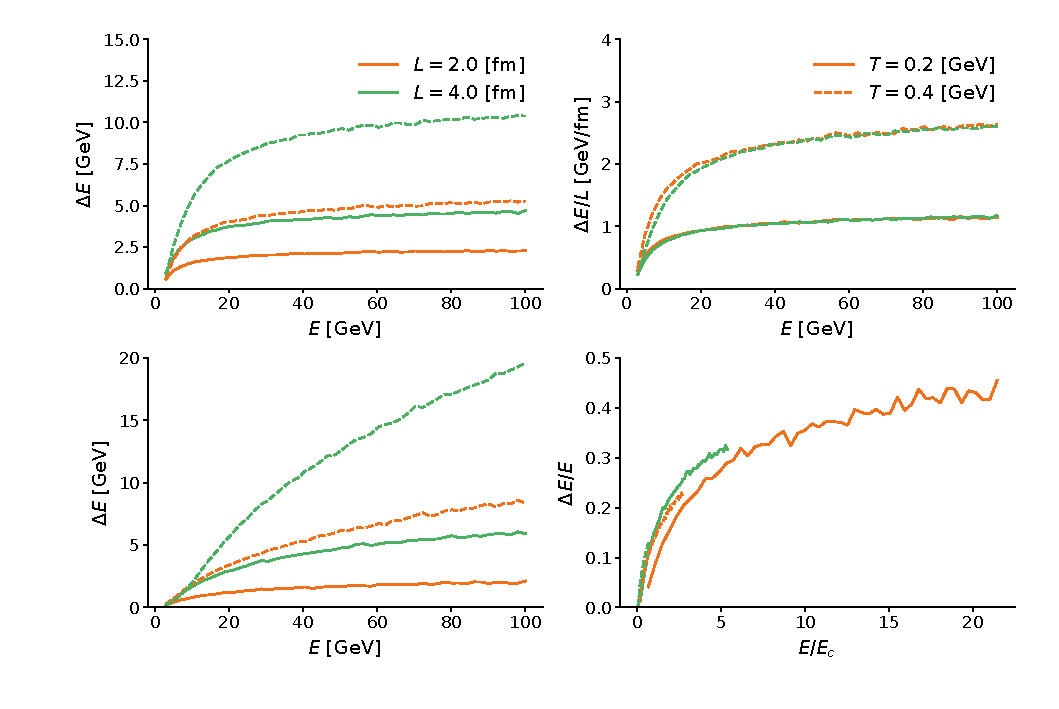
\includegraphics[width=\textwidth]{E_Eloss.pdf}
\caption{}\label{plots:dE-E}
\end{figure*}

\begin{figure*}
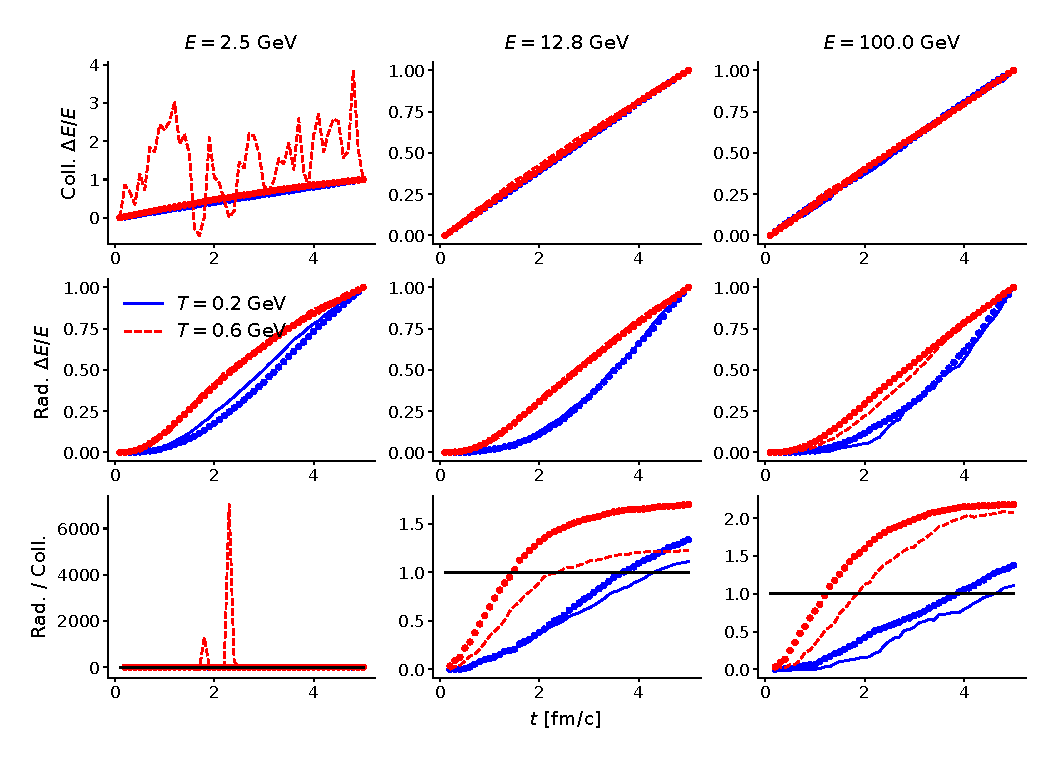
\includegraphics[width=\textwidth]{L_Eloss.pdf}
\caption{}\label{plots:dE-L}
\end{figure*}

\begin{figure}
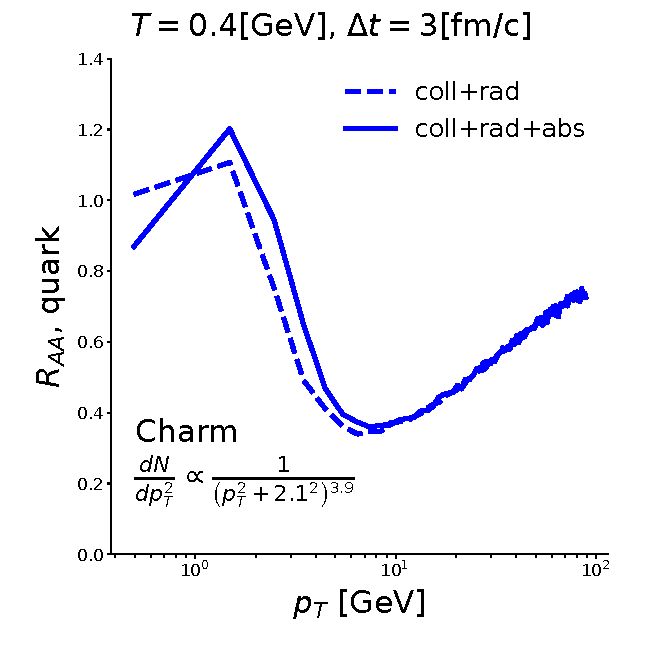
\includegraphics[width=\columnwidth]{BoxRaa.pdf}
\end{figure}

We first show our implementation of the above model gives the correct thermal limit. 
The quantify the approach to equilibrium of an ensemble of heavy quarks in side a static medium with a fixed temperature $T_0$, we define the following quantity,
\begin{eqnarray}
\Delta S = \frac{1}{N}\sum_i \ln f_0(E_i) - \int f_0(p)\ln f_0(p) dp^3
\end{eqnarray}
$f_0 \propto \exp(-E/T)$ is the relativistic Boltzmann distribution function at temperature $T$. 
The second term is the entropy at that temperature, while the first term is the ensemble average of one-particle entropy at that temperature.
This difference $\Delta S$ defines a ``distance" towards the equilibrium state, and vanishes when the thermal equilibrium is reached.
If the ensemble is not far from thermal equilibrium and can be characterized by an effective temperature $T_{\textrm{eff}}$ that the distribution function $f(E)\sim \exp(-E/T_{\textrm{eff}})$, then
\begin{eqnarray}
\nonumber
\Delta S &\sim& \frac{1}{T}\int  e^{-E/T_{\textrm{eff}}} E dp^3 - \frac{1}{T}\int e^{-E/T} E dp^3 \\
&=& \frac{T_\textrm{eff}-T}{T}
\end{eqnarray}
is an estimate of the deviation of the effective temperature from the temperature of the thermal bath.
Figure \ref{plots:thermalization} shows the time-evolution of $Delta S$ of heavy quarks inside thermal bath $T=0.4$ GeV with initial energy $E_0 = 10$ GeV.
With elastic process only, the system thermalize after about $150$ fm/$c$.
If we further turn on radiation process, the equilibrium is reached in a shorter amount of time, but it is wrong equilibrium.
The effective temperature is lower than the temperature of the thermal bath.
This is the consequence from breaking detailed balance with radiation process only.
By adding the absorption processes, the correct equilibrium is reached.
We also point out that the inclusion of absorption processes only start to make difference when the system is not far from equilibrium.

We can integrate collision rates using Equations \ref{eq:rate}, and calculate energy loss of a heavy quark by inserting $\Delta E$ into the integration of differential rates.
This is straight forward for elastic processes, but since the rates of inelastic processes depend on collision history, a meaningful rate and energy loss in side a medium can only be obtained by an actually Monte Carlo simulation.
Moreover, this history dependence is the reason that our rates and energy loss is not only a function of the incident energy ($E$) and medium temperature ($T$) but also the medium size (path length $L$).

In Figure \ref{plots:dE-E}, we plot energy loss fraction $\Delta E/E$ for elastic process (first row) and inelastic process (second row) as function of $E$ for different path length and temperature.
The elastic energy loss fraction increases as temperature and decreases for large energy.
At low energy, the heavy quark starts to gain net energy from the medium as which manifests as $\Delta E < 0$.
For the case of inelastic energy loss, we study the effect of gluon absorption process by comparing $\Delta E/E$ with radiation process only and with both radiation and absorption processes.
We find that gluon absorption process does not affect the energy loss at low temperature or high energy heavy quark as expected.
For high temperature such as $T=0.6$ GeV and energy below $10$ GeV, the gluon absorption process makes a notable difference.
Radiation process always leads to a positive average energy loss, but with absorption process, heavy quarks with very low energy actually on average gain energy from the medium.

In Figure \ref{plots:dE-L}, we show the path length dependence of the two energy loss mechanism.
Here, we plot the energy loss fraction per unit length, with length measured in units of inverse temperature.
The key observation is that elastic energy loss per unit length is a constant while for inelastic energy loss, this quantity first increases from zero for small path length and then gradually approaching a limit for large path length, showing a different medium size dependence of energy loss from the elastic process.
The non-linear path length dependence $\Delta E \propto L^2$ is actually a characteristic behavior of the coherence effect in a finite length medium [CITE]. 
In our effective implementation of LPM, this behavior arises because gluon radiation with
\begin{eqnarray}
\tau_f \ll L.
\end{eqnarray}
is suppressed, and therefore the inelastic energy loss for a thin medium is very small.
As $L$ increases, a high energy heavy quark could have radiated gluons with formation time $\tau_f$ multiples times $N \propto L/\tau_f$ where each radiation carries off a typical amount of energy. 
As a result the energy loss grows again linearly with path length.

Finally, for our study in a static medium, we calculate the $R_{AA}$ of charm and bottom quark in a medium $T=0.4$ GeV after evolving $3$ fm/c.
Here we initialize the charm quark spectra with the parametrization provided by [cite].
The heavy quarks looses a significant amount of energy in this static medium setup.
Again, we see that the gluon absorption process only affects $R_{AA}$ for relatively low momentum $p_T < 10$ GeV.
The mass plays an important role in the intermediate $p_T$ region.


\section{Calibration of the model at LHC using Bayesian analysis}\label{section:calibration}
This hybrid transport model contains three parameters right now ($\mu$ for scattering component and $A$ and $B$ for diffusion component).
By systematic comparison to experimental measurements of heavy-flavors in AA collisions, one can extract the these parameters with uncertainties.
The calculation of heavy flavor observables requires a multi-stage modeling including
\begin{itemize}
\item The soft medium production and evolution modeling.
\item Initial production spectra of heavy quarks (HQ).
\item HQ energy loss in the pre-equilibrium stage.
\item HQ energy loss in the quark-gluon plasma phase.
\item HQ hadronization.
\item HQ energy loss in the hadronic phase.
\end{itemize}


\begin{figure}
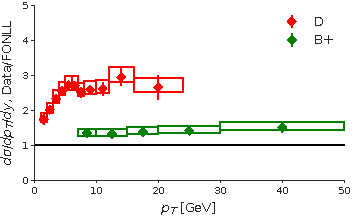
\includegraphics[width=\columnwidth]{baseline.pdf}
\caption{...}\label{plots:baseline}
\end{figure}

\begin{figure}
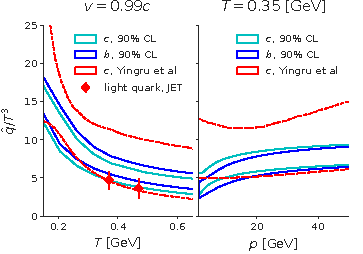
\includegraphics[width=\columnwidth]{qhat_p_T.pdf}
\caption{...}\label{plots:posterior_qhat}
\end{figure}

\begin{figure}
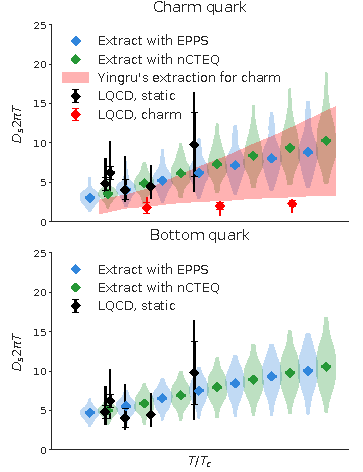
\includegraphics[width=\columnwidth]{Ds_posterior.pdf}
\caption{...}\label{plots:posterior_Ds}
\end{figure}


\begin{figure*}
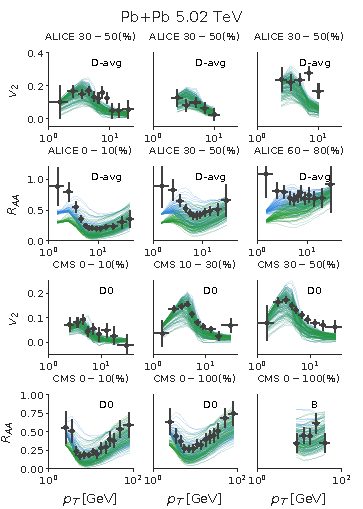
\includegraphics[width=.49\textwidth]{observables_design.pdf}
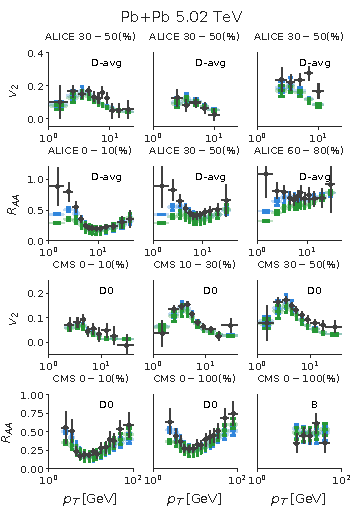
\includegraphics[width=.49\textwidth]{observables_posterior.pdf}
\caption{...}\label{plots:deisgn_posterior_obs}
\end{figure*}


\section{Calibration of the model at LHC using Bayesian analysis}\label{section:prediction}

\begin{figure*}
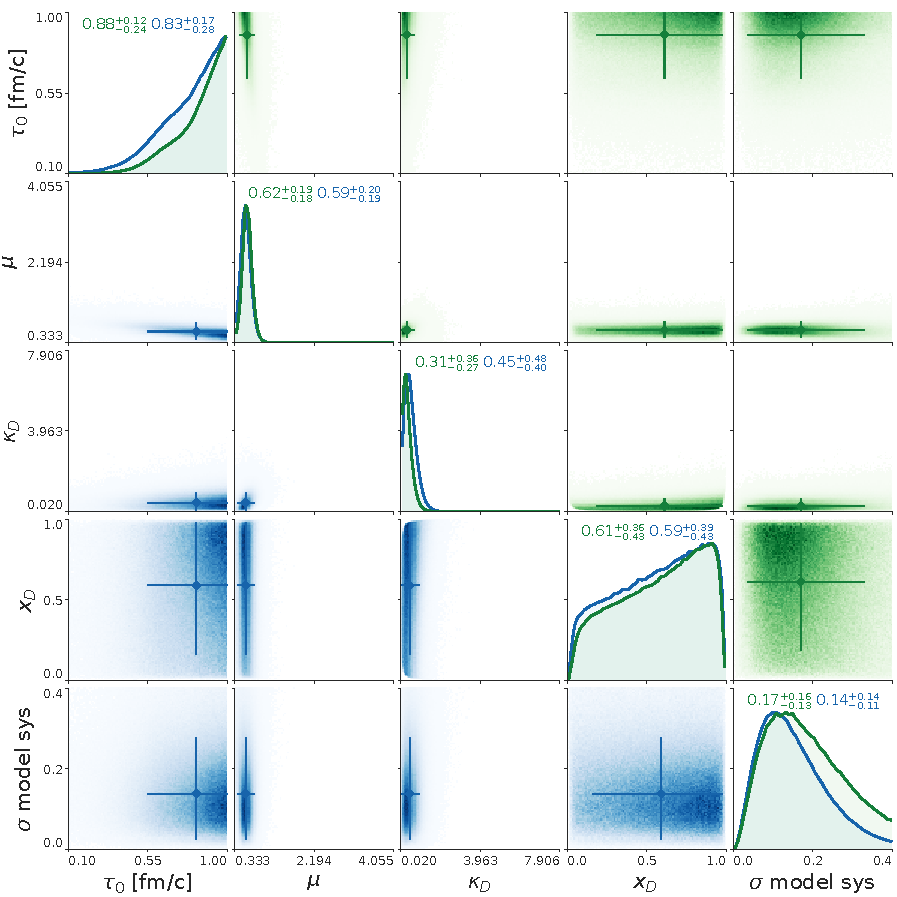
\includegraphics[width=\textwidth]{posterior.pdf}
\caption{...}\label{plots:posterior}
\end{figure*}
\begin{figure*}
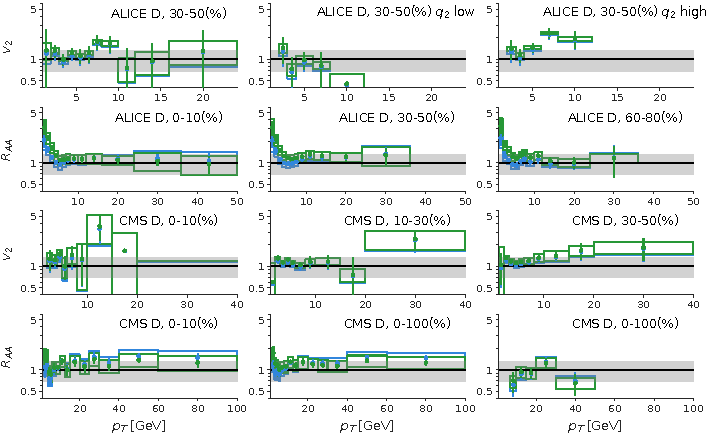
\includegraphics[width=\textwidth]{find_map.pdf}
\caption{...}\label{plots:posterior}
\end{figure*}

\section{Conclusion}\label{section:conclusion}


\begin{appendices}
\section{Running coupling}
We use the leading order running coupling constant with three flavors of quark,
\begin{eqnarray}
\alpha_s(Q^2) = \frac{4\pi}{9 \ln\left(Q^2/\Lambda^2\right) }
\end{eqnarray}
The QCD scale is set at $\Lambda = 0.2$~GeV.
Inside a medium, the temperature $T$ defines the medium scale, it is used as a lower cutoff for $Q^2$ of all process, and the running coupling is actually,
\begin{eqnarray}
\alpha_s = \alpha_s(\max\{Q^2,(\mu T)^2\})
\end{eqnarray}
$\mu$ the only parameter we tuned in the scattering component of the hybrid model.
For elastic scattering, $Q^2$ is chosen as the momentum exchange squared for $s,t,u$ channel.
For the gluon emission / absorption vertex, we choose $Q^2 = k_\perp^2$.


\section{Matrix elements}
\label{appendix:matrix-element}
\begin{widetext}
\begin{eqnarray}
\overline{|M_{Q+q\rightarrow Q+q}|^2} &=& \frac{64\pi^2}{9}\alpha_s^2 \frac{(u-M^2)^2 + (s-M^2)^2 + 2 M^2 t}{(t-m_D^2)^2}
\end{eqnarray}
\begin{eqnarray}
\overline{|M_{Q+g\rightarrow Q+g}|^2} &=& \pi^2 \left\{
32\alpha_s^2 \frac{(s-M^2)(-u+M^2)}{(t-m_D^2)^2} \right. \\ \nonumber
&+&\frac{64}{9}\alpha_s^2 \frac{(s-M^2)(-u+M^2)+2M*2(s-M^2) + 4M^4}{(s-M^2+m_D^2)^2} \\ \nonumber
&+&\frac{64}{9}\alpha_s^2 \frac{(s-M^2)(-u+M^2)+2M*2(u-M^2) + 4M^4}{(-u+M^2+m_D^2)^2} \\ \nonumber
&+&\frac{16}{9}\alpha_s^2 \frac{M^2(4M^2 - t)}{(-u+M^2+m_D^2)(s-M^2+m_D^2)} \\ \nonumber
&+& 16 \alpha_s^2 \frac{(s-M^2)(-u+M^2)+M^2(s-u)}{(t-m_D^2)(s-M^2+m_D^2)} \\ \nonumber
&-& \left. 16 \alpha_s^2 \frac{(s-M^2)(-u+M^2)-M^2(s-u)}{(t-m_D^2)(-u+M^2+m_D^2)}\right\} 
\end{eqnarray}
\begin{eqnarray}
\frac{\overline{|M_{Q+q\rightarrow Q+q+g}|^2}}{\overline{|M_{Q+q\rightarrow Q+q}|^2}} &=&  \frac{\overline{|M_{Q+g\rightarrow Q+g+g}|^2}}{\overline{|M_{Q+g\rightarrow Q+g, \textrm{t-channel}}|^2}} = P_g
\end{eqnarray}
\begin{eqnarray}
P_g = 48 \pi \alpha_s (1-\bar{x})^2 \left(\frac{\vec{k}_\perp}{k_\perp^2 + x^2 M^2 + (1-\bar{x})\mu^2} 
+ \frac{\vec{q}_\perp - \vec{k}_\perp}{(\vec{q}_\perp-\vec{k}_\perp)^2 + x^2 M^2 + (1-\bar{x})\mu^2}
\right)^2 
\end{eqnarray}
\end{widetext}

\section{Evolution with both scattering and diffusion dynamics}
With a transport $\hat{T} = -v\cdot \partial_x$, a scattering $\hat{C}$, and a diffusion $\hat{D}$ operator in the hybrid transport equation,
\begin{eqnarray}
\frac{\partial f}{\partial t} = \left( \hat{T} + \hat{C} + \hat{D} \right) f
\end{eqnarray}
The formal solution is,
\begin{eqnarray}
f_{\Delta t} = e^{\int_0^{\Delta t}  \left( \hat{T} + \hat{C} + \hat{D} \right) dt}f_0
\end{eqnarray}
Assume the time variance of the medium are slow and decompose the joint operation into separate operations.
\begin{eqnarray}
e^{ \Delta t\left(\hat{T} +\hat{C} + \hat{D} \right)} &=&
\nonumber
e^{\Delta t \left(\hat{T} + \hat{D}\right) } e^{\Delta t \hat{C}}   e^{-\frac{\Delta t^2}{2} [\hat{T}+\hat{D}, \hat{C}]}\left(1+O(\Delta t^3)\right) \\
\nonumber
&=& \frac{1}{2}  \left\{
1+\Delta t \left( \hat{T}+\hat{D} \right), 1+\Delta t C
\right\} + O(\Delta t^3) 
\end{eqnarray}
The operator $1 + \Delta t ( \hat{T}  + \hat{D} )$ stands for a ``Diffusion" step in the simulation; the operator $1+\Delta t \hat{C}$ stands for a ``Scattering" step in the simulation. 
Therefore, we design the following simulation procedure.
\begin{itemize}
\item For each step, choose a $\Delta t$ in lab frame small enough that total scattering probability $P_c \ll 1$.
\item Determine the ordering of diffusion step and scattering step with 50-50\% chance
\item If diffusion operates before scattering.
\begin{itemize}
\item[Step 1.] $(t, x, p) \xrightarrow{\textrm{Diffusion}} (t+\Delta t, x', p^*)$.
\item[Step 2.] $(t+\Delta t, x', p^*) \xrightarrow{\textrm{Scattering}} (t+\Delta t, x', p')$.
\end{itemize}
\item If diffusion operates after scattering.
\begin{itemize}
\item[Step 1.] $(t, x, p) \xrightarrow{\textrm{Scattering}} (t, x, p^*)$.
\item[Step 2.] $(t, x, p^*)  \xrightarrow{\textrm{Diffusion}} (t+\Delta t, x', p')$.
\end{itemize}
\end{itemize}

\section{Calculation of $v_n\{2\}$ and $v_2\{EP\}$}
Cumulant method correlates a heavy meson with a light particle to estimate $v_n$. 
\begin{eqnarray}
v_n\{2\} &=& \frac{d_n\{2\}}{\sqrt{c_n\{2\}} } \\
d_n\{2\} &=& \left\langle \frac{\Re\{pQ^*\}}{mM} \right\rangle_{w = mM} \\
c_n\{2\} &=& \left\langle \frac{|Q|^2-M}{M(M-1)} \right\rangle_{w = M(M-1)}
\end{eqnarray}
\end{appendices}
\end{document}